\documentclass[margin = 0.5cm]{standalone}

\usepackage{mathtools}
\usepackage{tikz}
\usetikzlibrary{positioning, arrows.meta}

\tikzset{> = { Latex[length = 2.5mm] }}

\renewcommand{\vec}[1]{\boldsymbol{#1}}

\begin{document}
	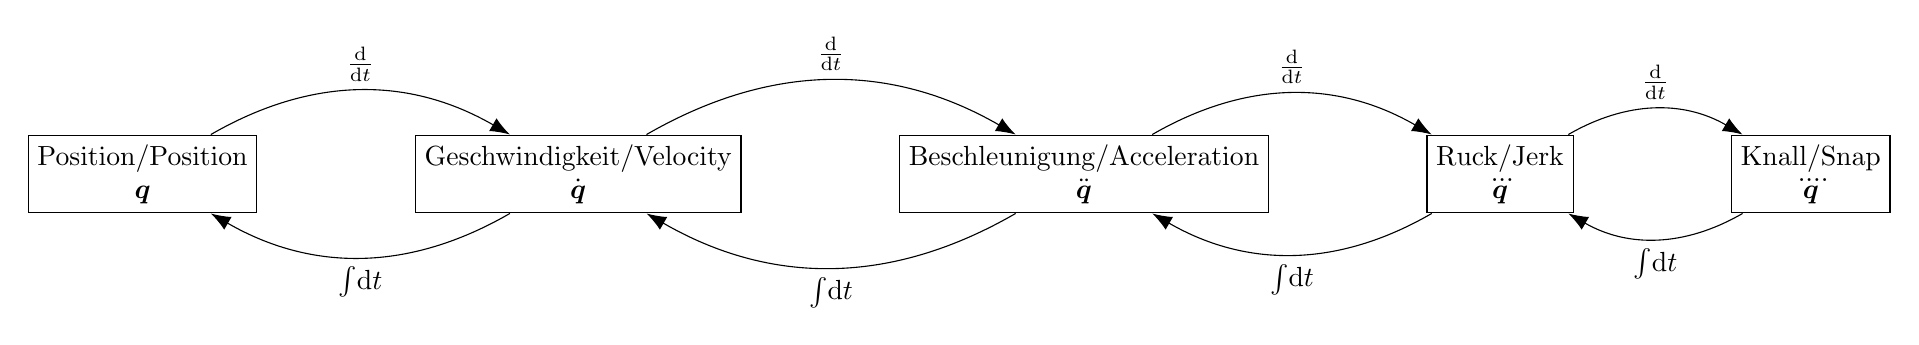
\begin{tikzpicture}[every node/.style = { align = center }]
		\node [draw, rectangle] (position) { Position/Position \\ \( \vec{q} \) };
		\node [draw, rectangle, right = 2 of position] (velocity) { Geschwindigkeit/Velocity \\ \( \dot{\vec{q}} \) };
		\node [draw, rectangle, right = 2 of velocity] (acceleration) { Beschleunigung/Acceleration \\ \( \ddot{\vec{q}} \) };
		\node [draw, rectangle, right = 2 of acceleration] (jerk) { Ruck/Jerk \\ \( \dddot{\vec{q}} \) };
		\node [draw, rectangle, right = 2 of jerk] (snap) { Knall/Snap \\ \( \ddddot{\vec{q}} \) };

		\draw [->] (position) to[bend left] node[above]{\( \frac{\text{d}}{\text{d}t} \)} (velocity);
		\draw [->] (velocity) to[bend left] node[above]{\( \frac{\text{d}}{\text{d}t} \)} (acceleration);
		\draw [->] (acceleration) to[bend left] node[above]{\( \frac{\text{d}}{\text{d}t} \)} (jerk);
		\draw [->] (jerk) to[bend left] node[above]{\( \frac{\text{d}}{\text{d}t} \)} (snap);

		\draw [->] (snap) to[bend left] node[below]{\( \int \! \text{d}t \)} (jerk);
		\draw [->] (jerk) to[bend left] node[below]{\( \int \! \text{d}t \)} (acceleration);
		\draw [->] (acceleration) to[bend left] node[below]{\( \int \! \text{d}t \)} (velocity);
		\draw [->] (velocity) to[bend left] node[below]{\( \int \! \text{d}t \)} (position);
	\end{tikzpicture}
\end{document}
